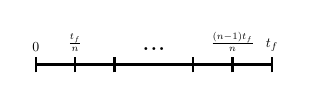
\begin{tikzpicture}
\draw[thick] (0,0) -- (3.0,0);
\draw[thick]	(0,-0.1) -- (0,0.1) node[anchor=south,scale=0.5] {$0$};
\draw[thick]	(0.5,-0.1)--(0.5,0.1) node[anchor=south,scale=0.5] {$\frac{t_f}{n}$};
\draw[thick]	(1.0,-0.1)--(1.0,0.1) ;
\foreach \Point in {(1.4,0.2), (1.5,0.2), (1.6,0.2)}{
    \node at \Point {.};
}
\draw[thick]	(2.0,-0.1)--(2.0,0.1) ;
\draw[thick]	(2.5,-0.1)--(2.5,0.1) node[anchor=south,scale=0.5] {$\frac{(n-1)t_f}{n}$};
\draw[thick]	(3.0,-0.1)--(3.0,0.1) node[anchor=south,scale=0.5] {$t_f$};
\end{tikzpicture}